% Figure snippets — copy images from repo: figures/paper/ and figures/qual_cvc_in/
% Requires: \usepackage{graphicx} \usepackage{subcaption} (optional)

\begin{figure*}[t]
  \centering
  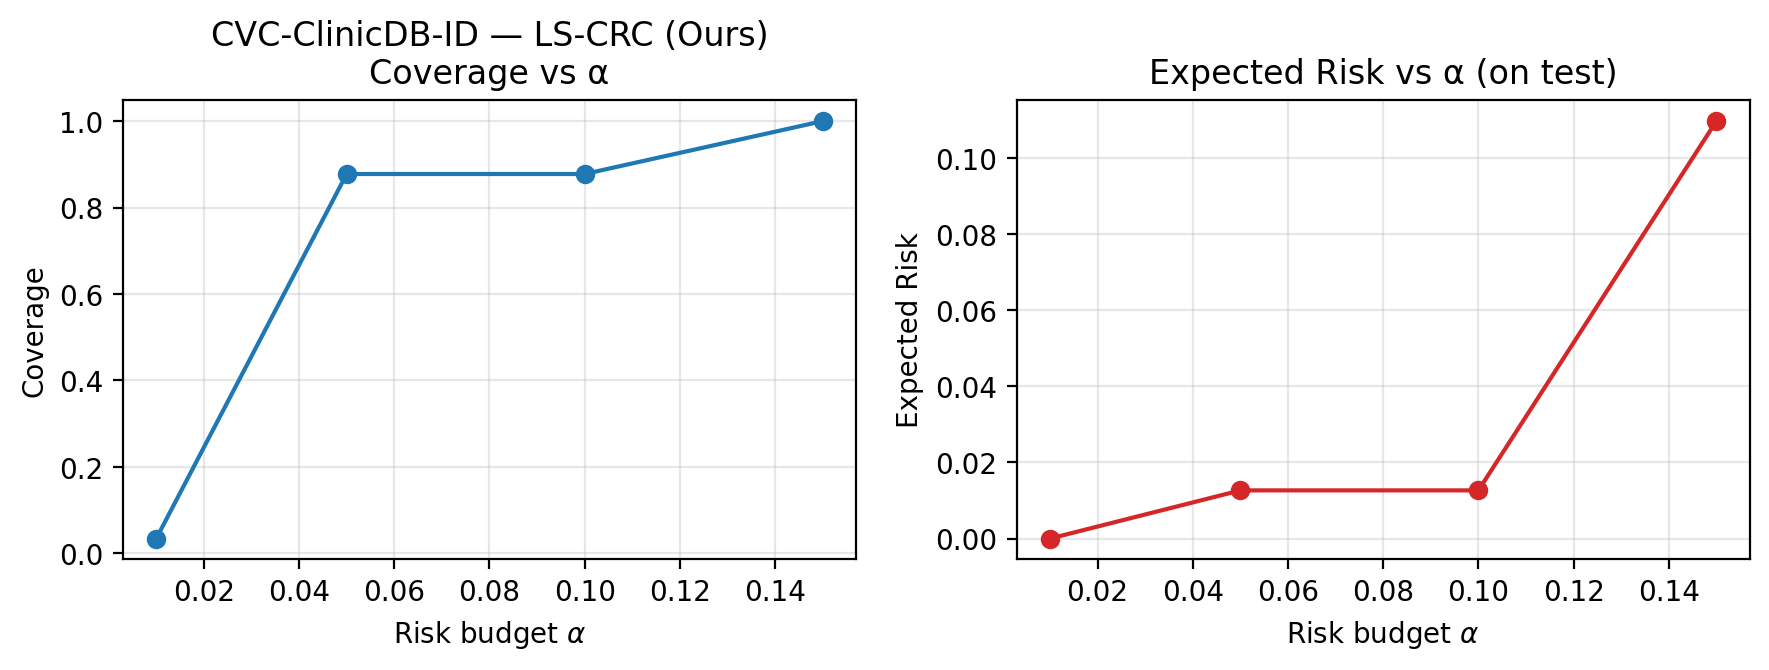
\includegraphics[width=\linewidth]{figures/paper/risk_coverage_vs_alpha__cvc__lscrc.png}
  \caption{Effect of risk budget $\alpha$ on mean coverage and mean localized expected risk for LS-CRC on the CVC-ClinicDB test set (in-domain calibration).}
  \label{fig:risk-coverage-vs-alpha}
\end{figure*}

\begin{figure}[t]
  \centering
  \includegraphics[width=0.85\linewidth]{figures/paper/risk_coverage_vs_alpha__cvc__lscrc_scatter.png}
  \caption{Mean coverage vs.\ mean localized expected risk for LS-CRC at several $\alpha$ (CVC in-domain).}
  \label{fig:risk-coverage-scatter}
\end{figure}

% Qualitative: pick one exported PNG, e.g. fig_qual_cvc_000.png
\begin{figure*}[t]
  \centering
  \includegraphics[width=\linewidth]{figures/qual_cvc_in/fig_qual_cvc_000.png}
  \caption{Qualitative example: input, ground truth, prediction overlay, and LS-CRC acceptance map after calibration ($\alpha=0.05$, CVC in-domain).}
  \label{fig:qualitative}
\end{figure*}
